
\begin{figure}[hp]
% 
\begin{subfigure}[t]{.5\linewidth}
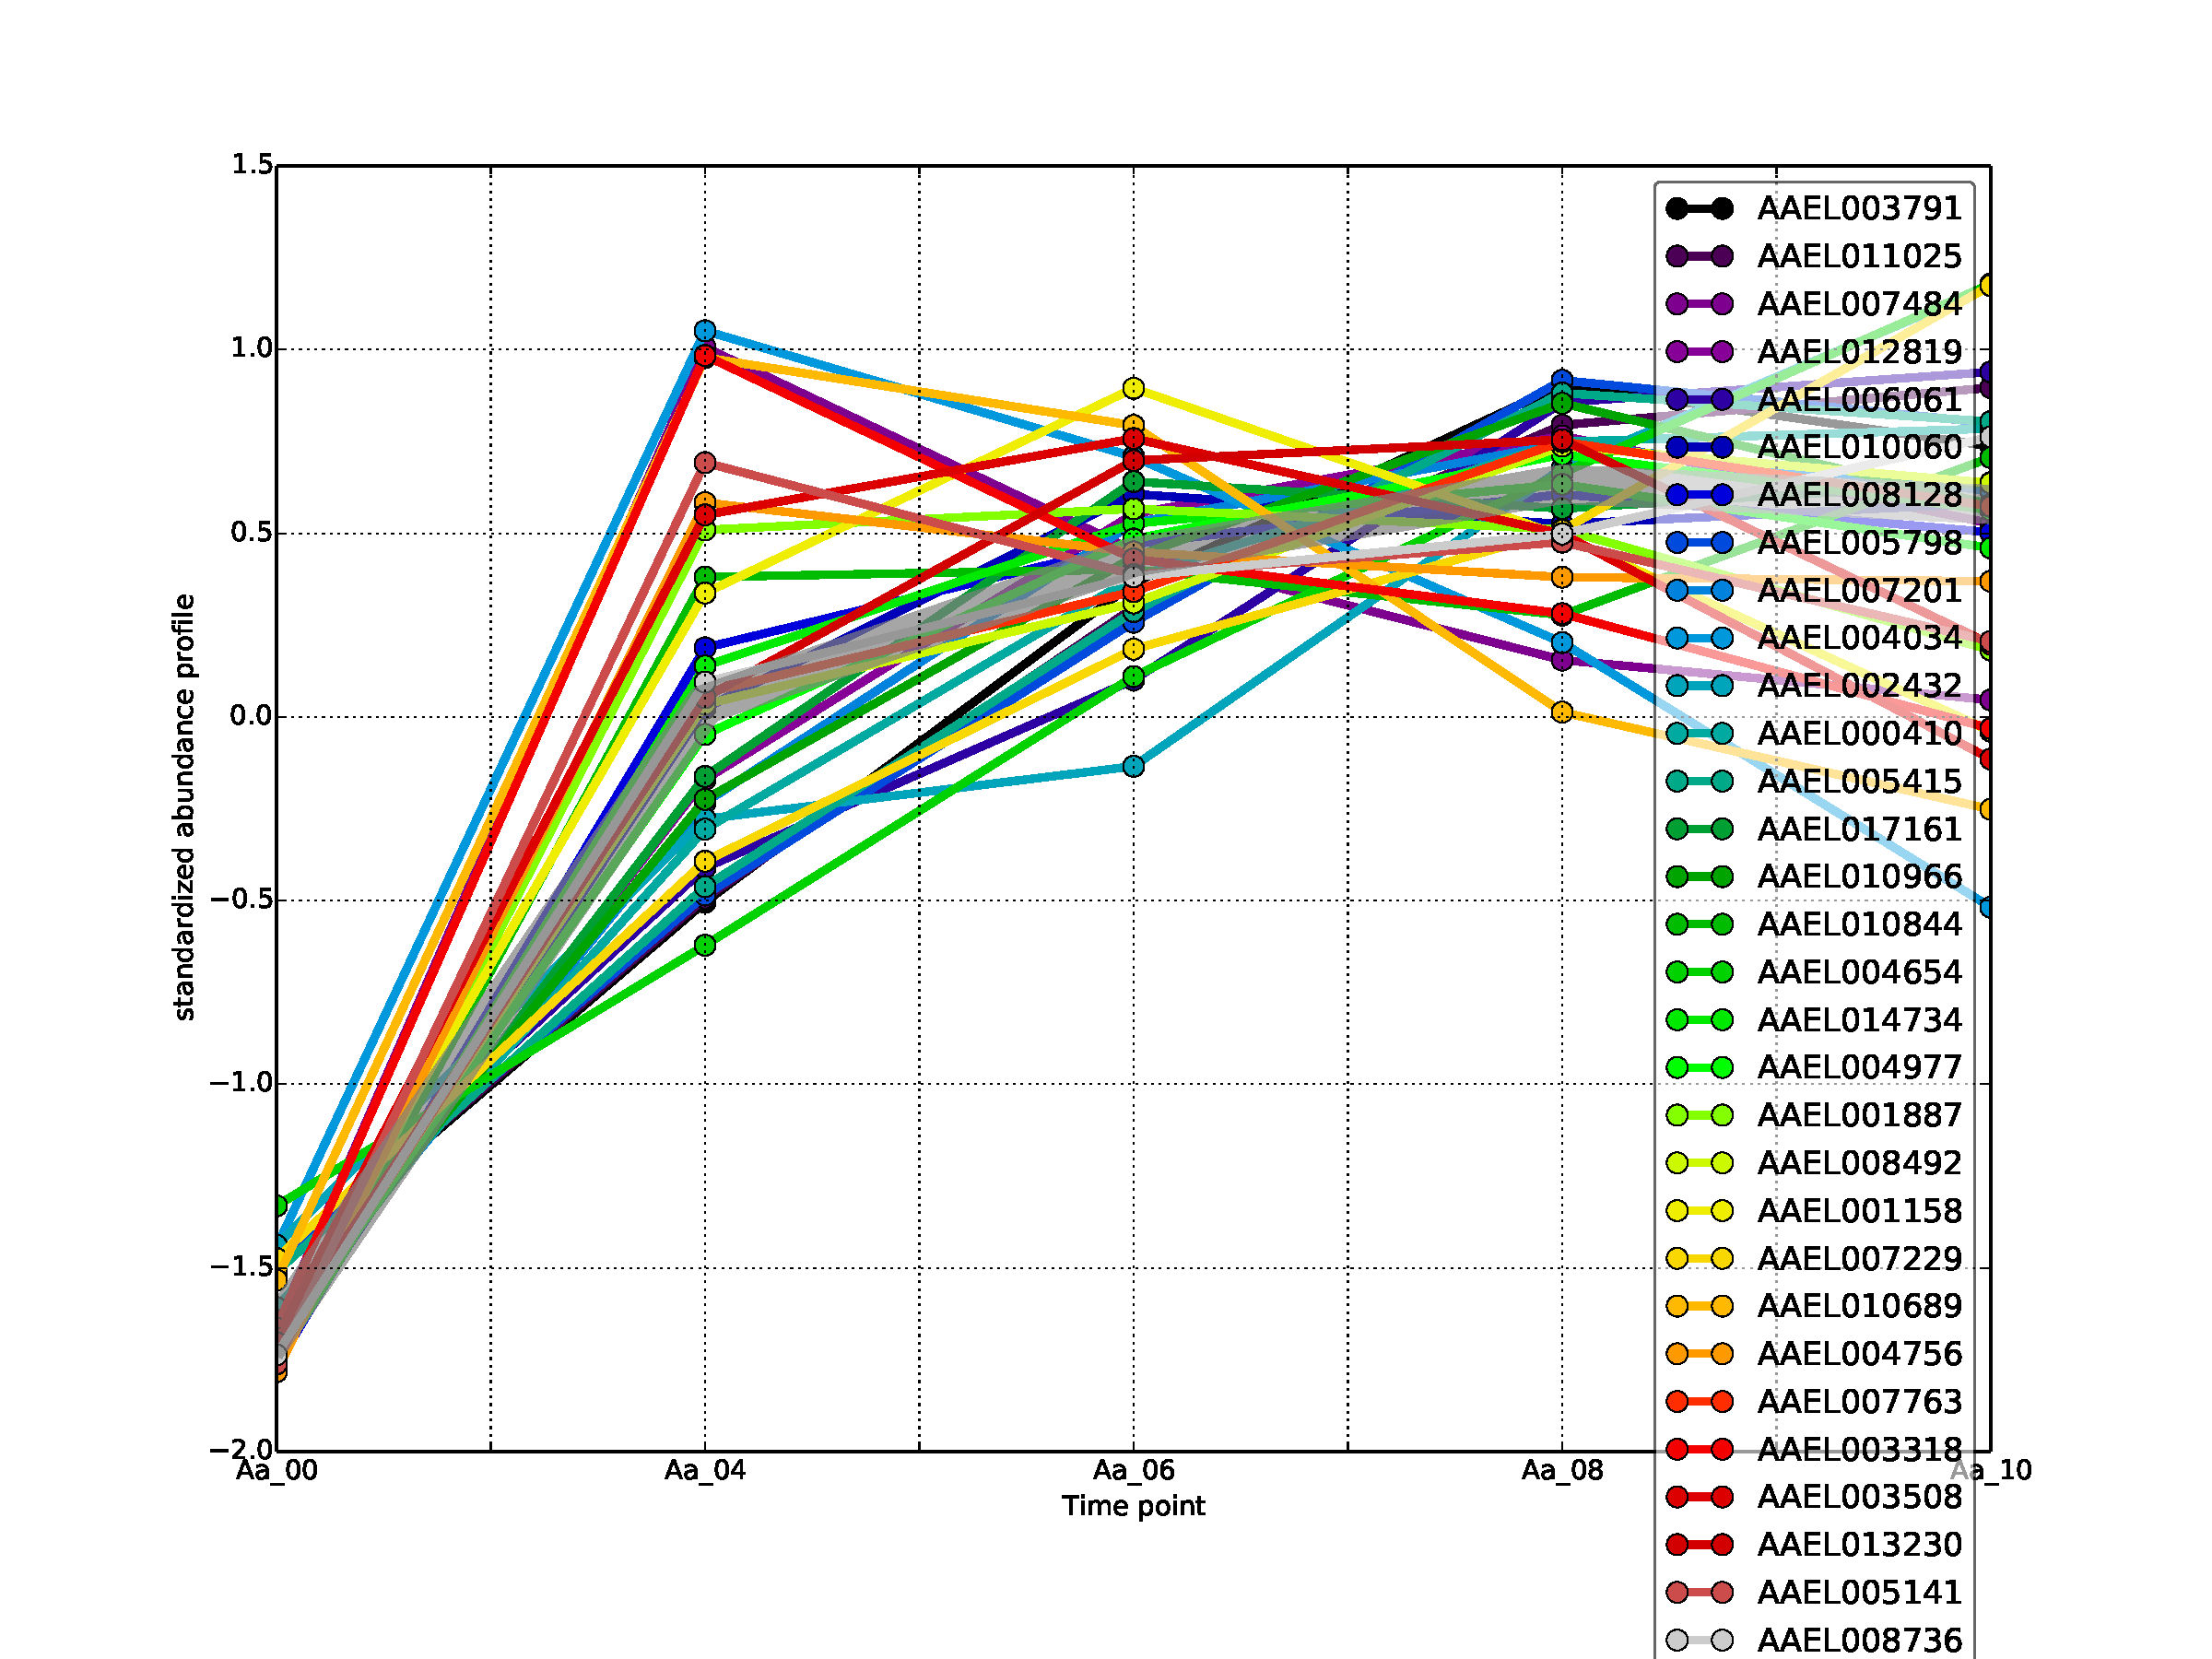
\includegraphics[width=\linewidth]{figures/figs/ecr_and_insects_ptci_20130903/upAfter4_gene_profiles_from_cummerbund/Aa_upAfter4_cls7_Ag_target_FPKMs_vb_orthos.pdf}
\caption{}
\label{fig:cluster7-Aa}
\end{subfigure}%
%
\begin{subfigure}[t]{.5\linewidth}
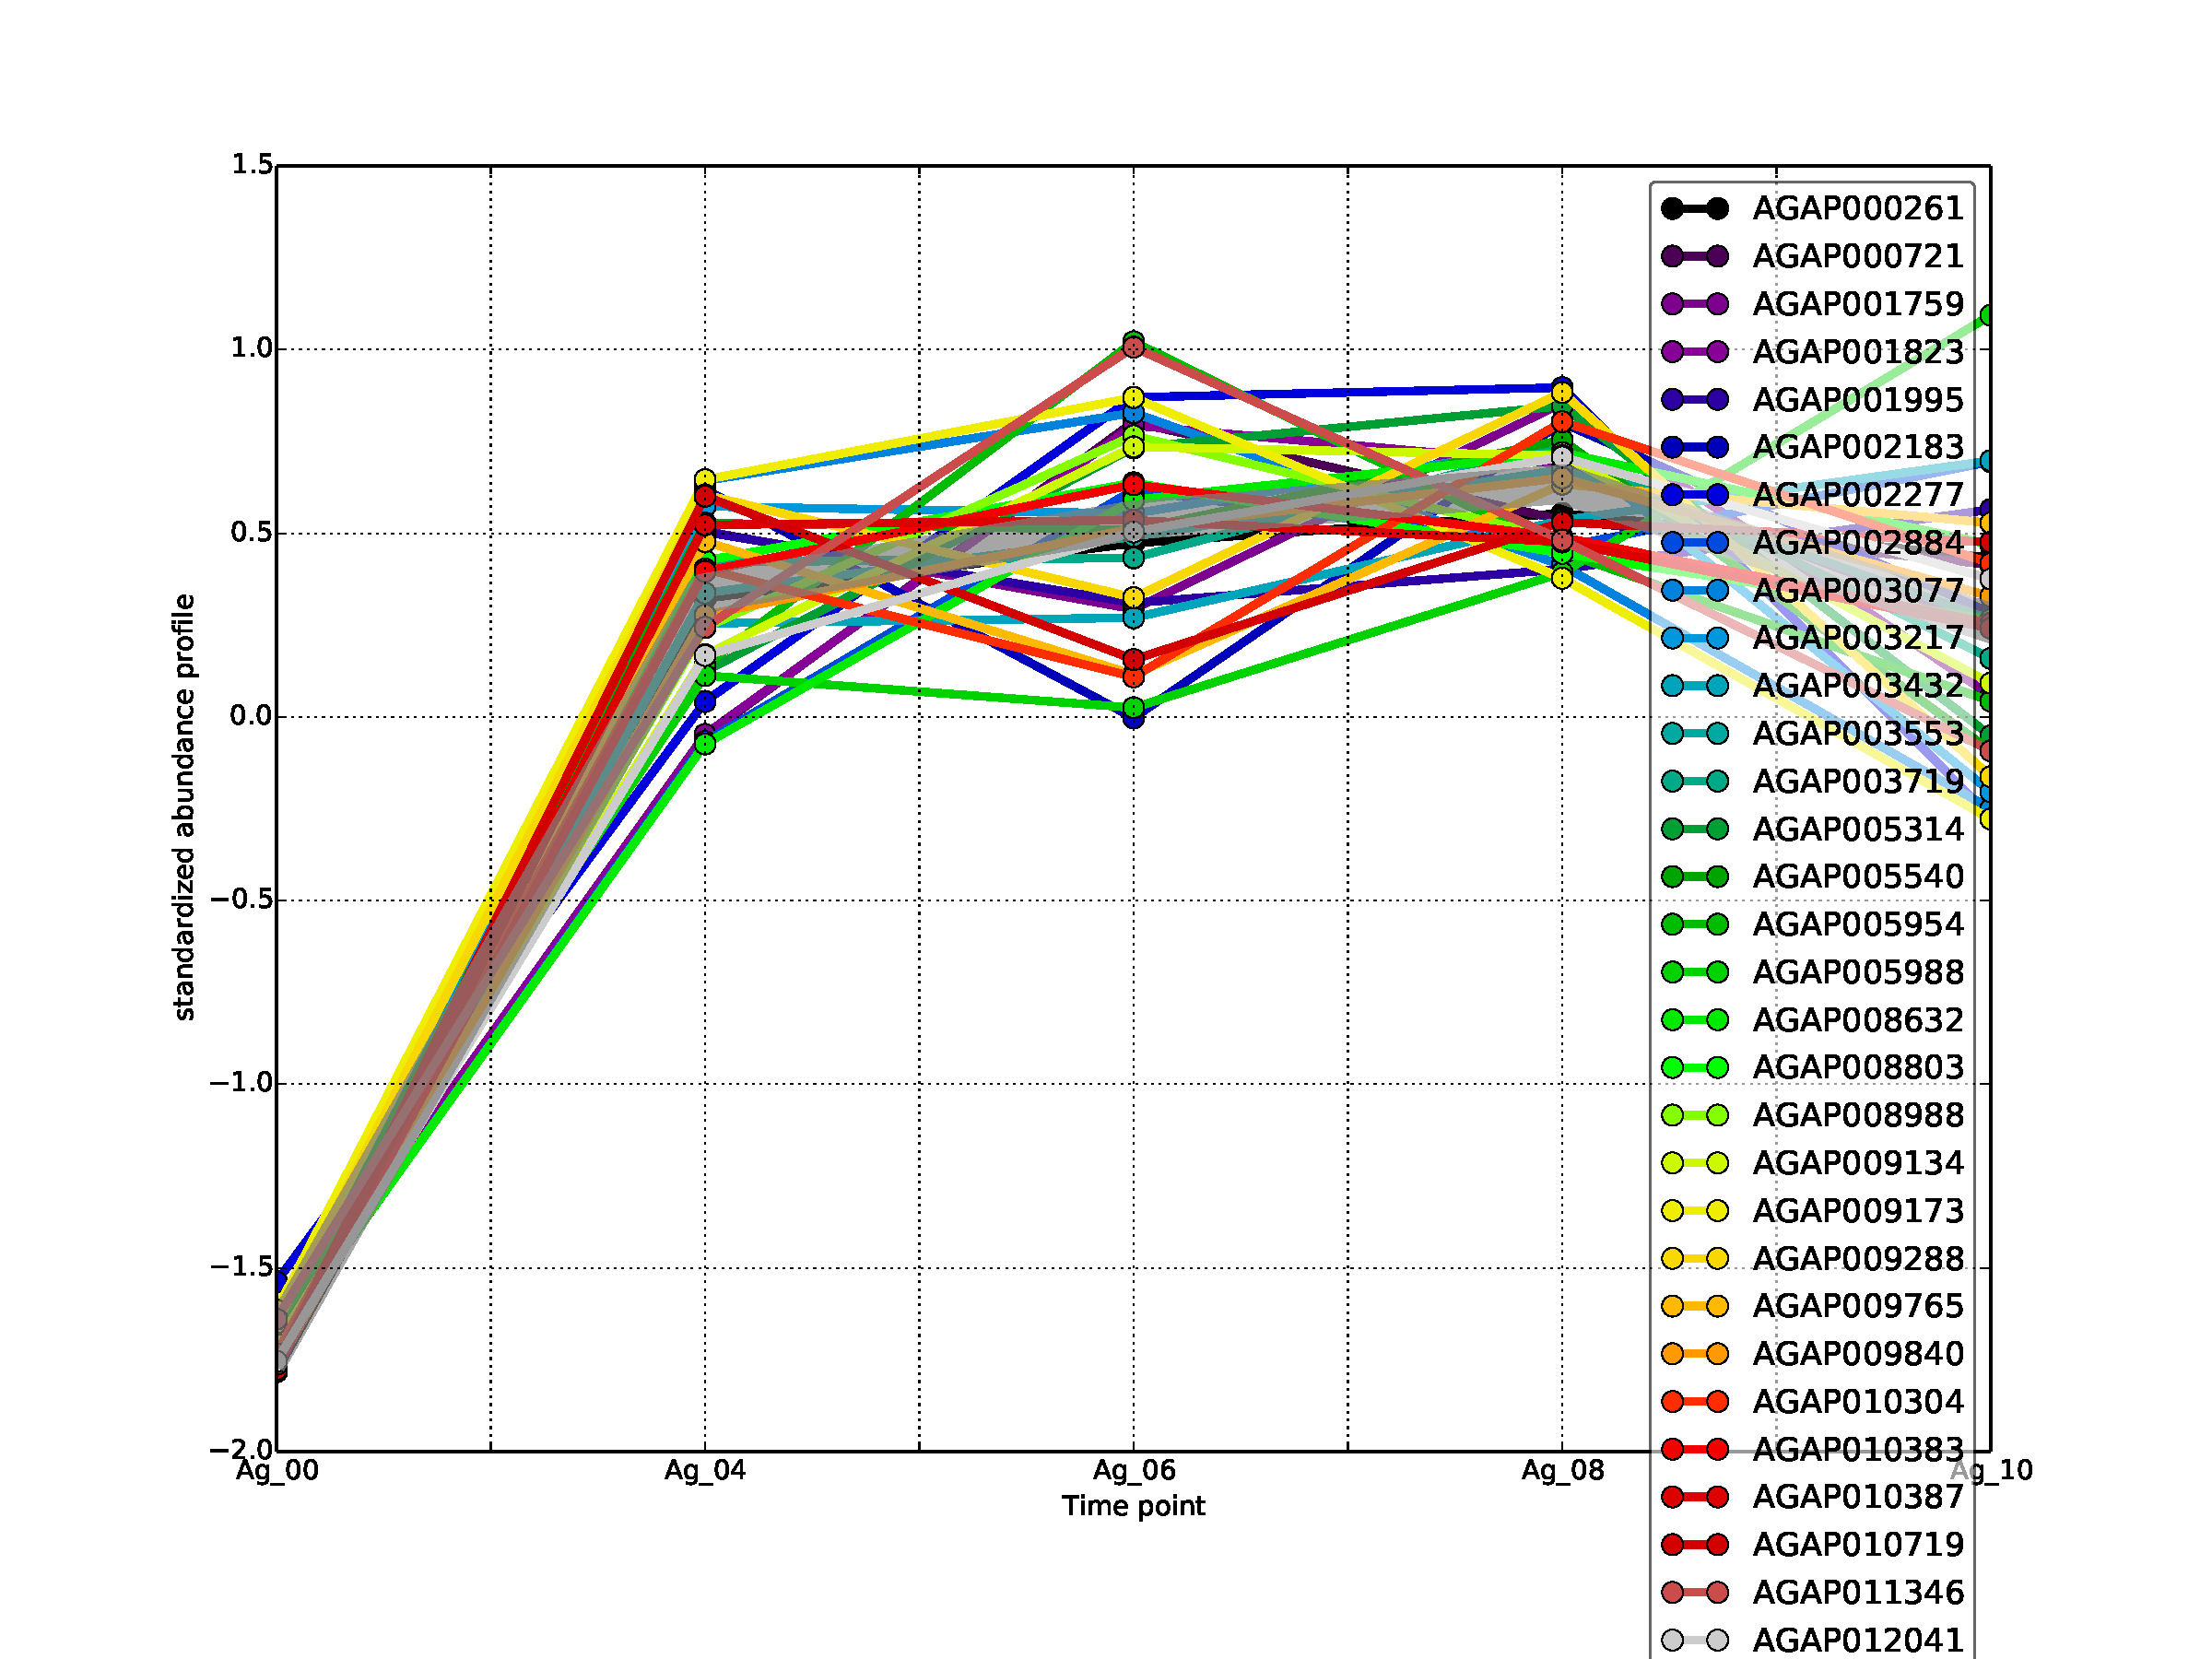
\includegraphics[width=\linewidth]{figures/figs/ecr_and_insects_ptci_20130903/upAfter4_gene_profiles_from_cummerbund/Ag_upAfter4_cls7_Ag_target_FPKMs_vb_orthos.pdf}
\caption{}
\label{fig:cluster7-Ag}
\end{subfigure}
% 
\begin{subfigure}[t]{.5\linewidth}
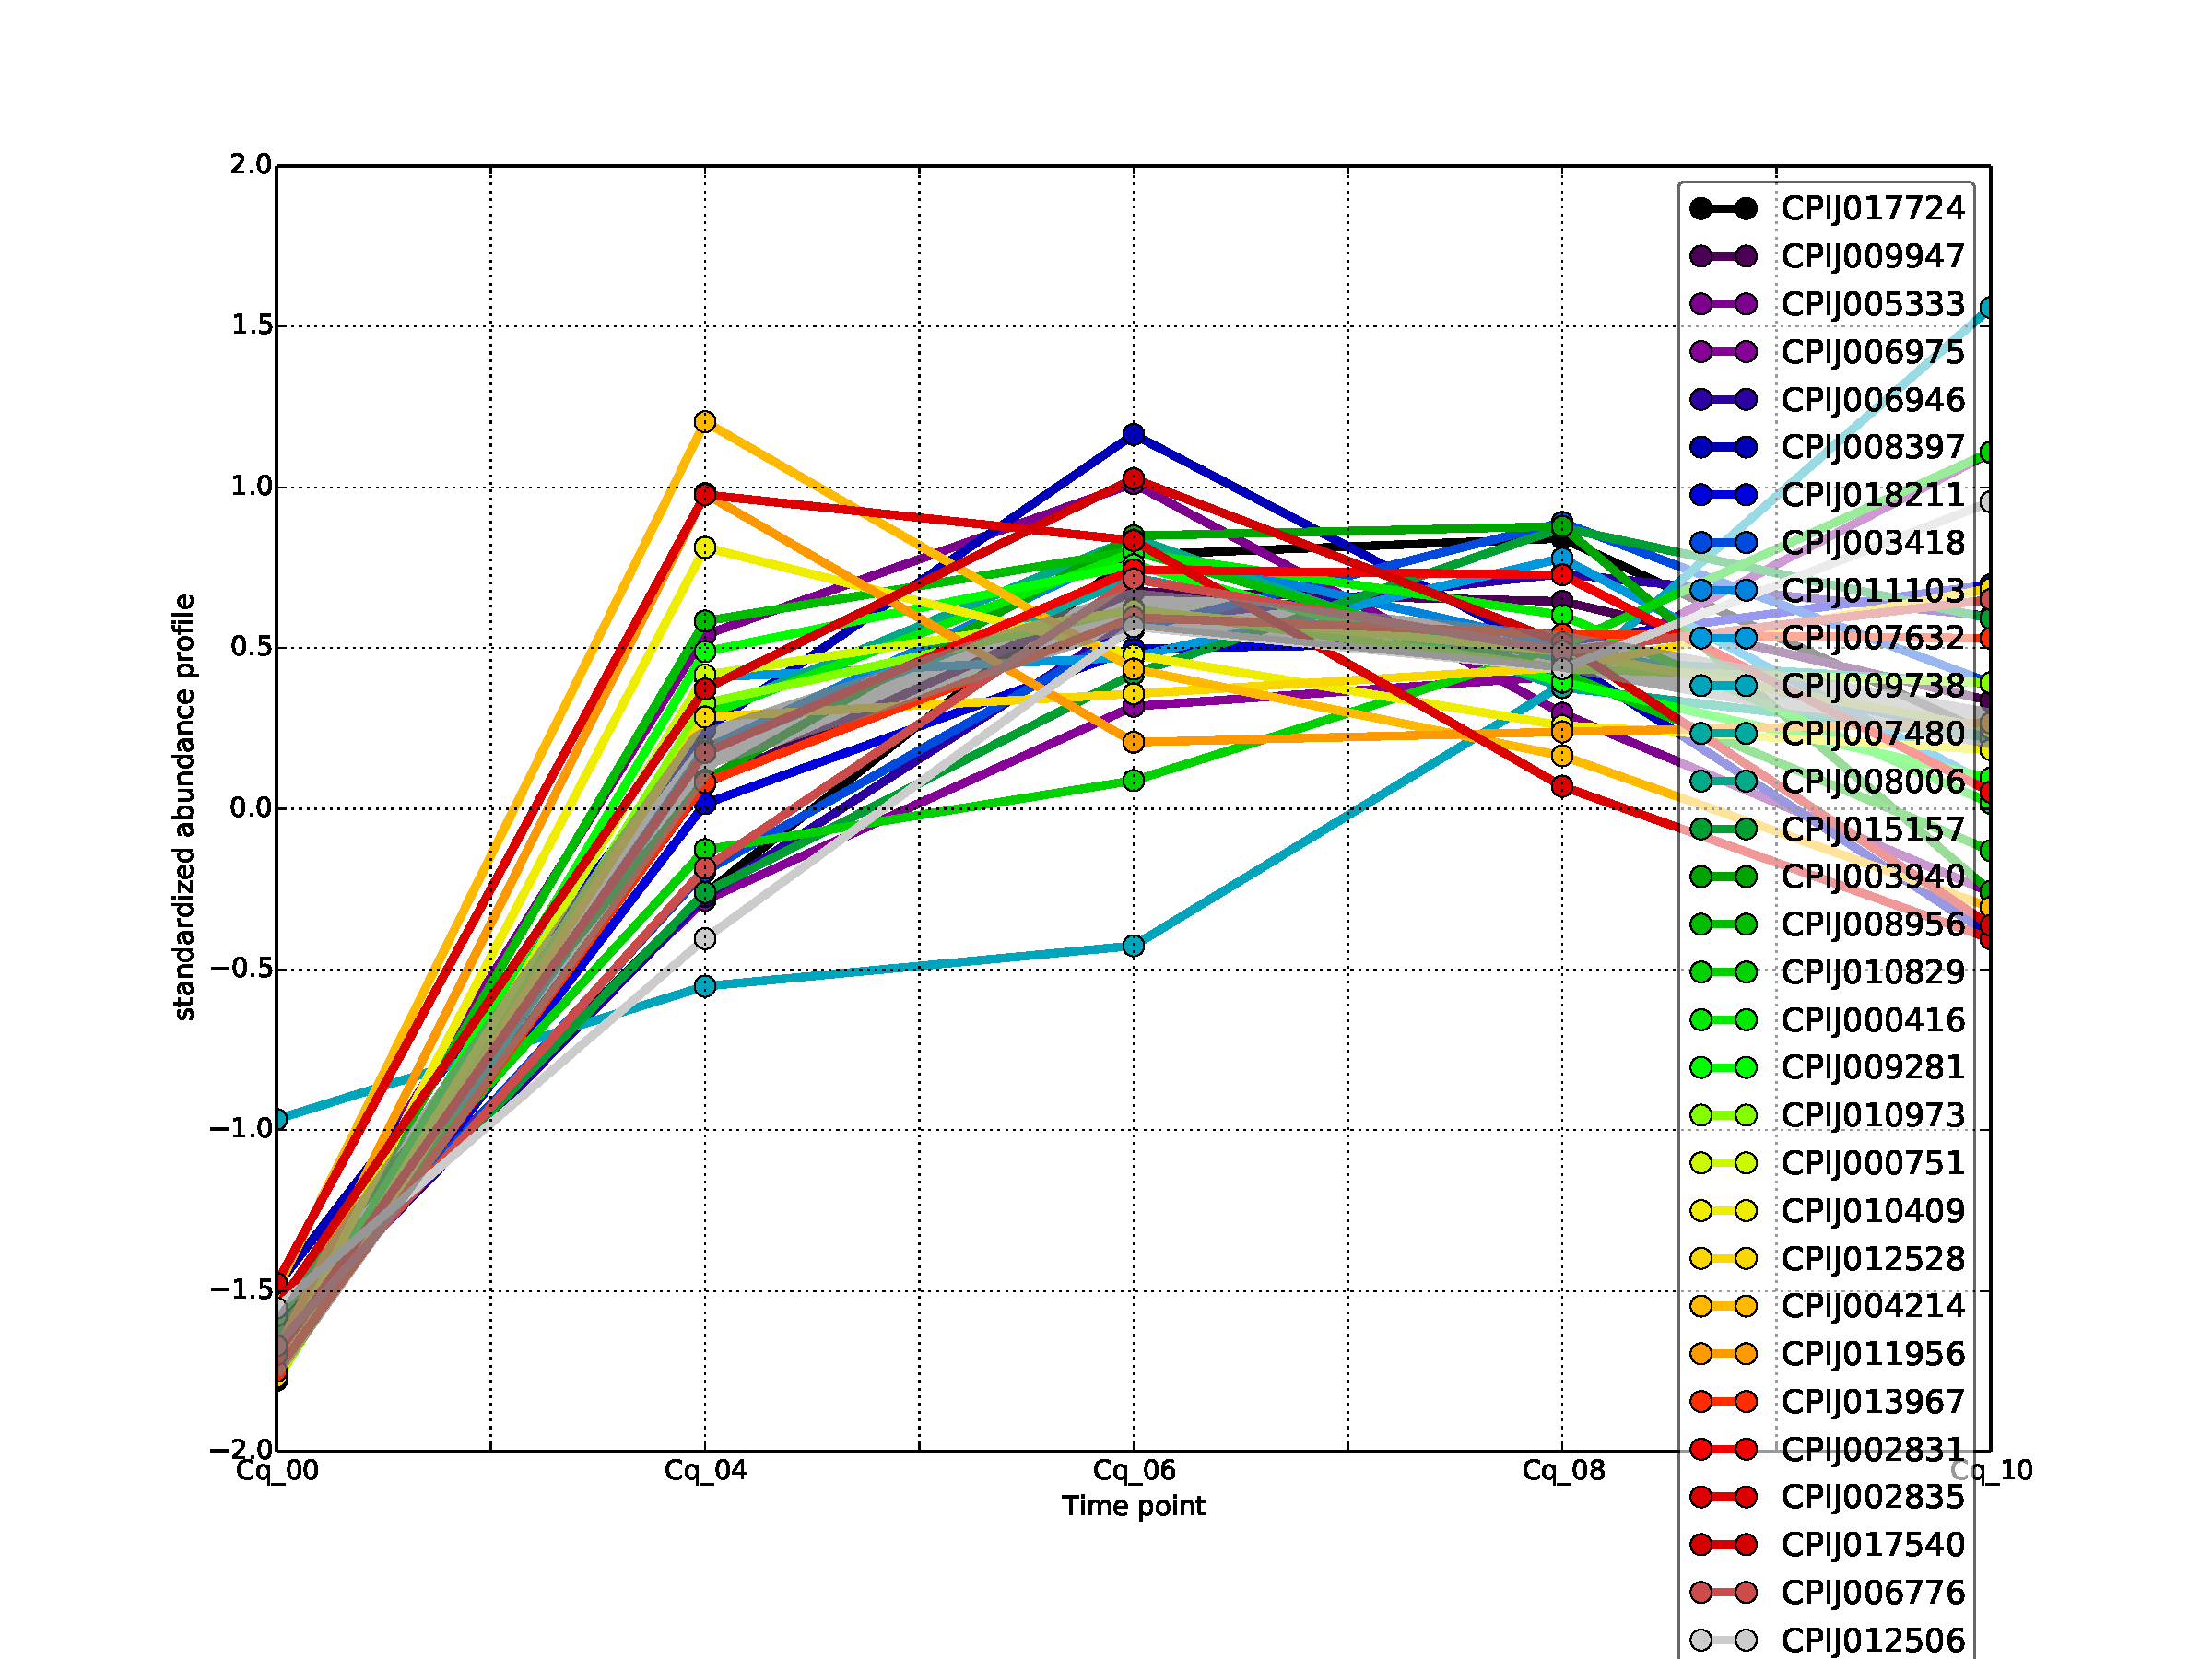
\includegraphics[width=\linewidth]{figures/figs/ecr_and_insects_ptci_20130903/upAfter4_gene_profiles_from_cummerbund/Cq_upAfter4_cls7_Ag_target_FPKMs_vb_orthos.pdf}
\caption{}
\label{fig:cluster7-Cq}
\end{subfigure}
% 
\caption[Orthologs of cluster 7]{\sf \textbf{Orthologs of cluster 7:}\\

\textbf{(A)} \Aa.
\textbf{(B)} \Ag.
\textbf{(C)} \Cq.
\todo[inline,caption={Finish Fig \ref{fig:cluster7}}]{ 
\begin{itemize}
    \item the text
    \item double gene names
    \item fix fig widths
\end{itemize}}
}
\label{fig:cluster7}
\end{figure}